\documentclass[tikz,border=3pt]{standalone}
\usepackage{tikz}
\usetikzlibrary{arrows.meta,positioning}

\begin{document}
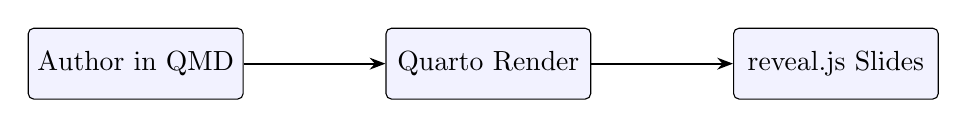
\begin{tikzpicture}[node distance=1.8cm]
  \tikzset{
    block/.style={draw, rounded corners=2pt, fill=blue!5, minimum width=2.6cm, minimum height=0.9cm},
    flow/.style={-{Stealth[length=2mm]}, line width=0.8pt}
  }

  \node[block] (author) {Author in QMD};
  \node[block, right=of author] (quarto) {Quarto Render};
  \node[block, right=of quarto] (slides) {reveal.js Slides};

  \draw[flow] (author) -- (quarto);
  \draw[flow] (quarto) -- (slides);
\end{tikzpicture}
\end{document}
